\begin{blocksection}
\question Write a function, \lstinline$replace_x$ that takes in a tree, \lstinline$t$, and returns a new tree with all
labels \lstinline$x$ replaced with 0.

For example, if we called \lstinline$replace_x(t, 2)$ on the following tree:

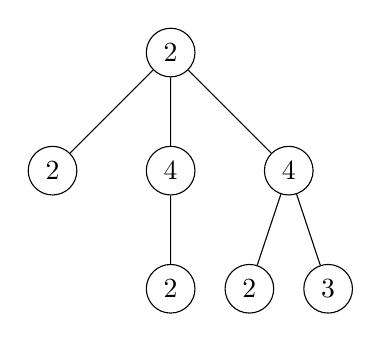
\begin{tikzpicture}[scale=1, transform shape]
\tikzstyle{level 2}=[sibling distance=10mm]
    \node [circle, draw] (z){$2$}
        child {node [circle, draw] (a) {$2$}}
        child {node [circle, draw] (d) {$4$}
            child {node [circle, draw] (g) {$2$}}
        }
        child {node [circle, draw] (b) {$4$}
            child {node [circle, draw] (e) {$2$}}
            child {node [circle, draw] (f) {$3$}}
        };
\end{tikzpicture}

We would expect it to return

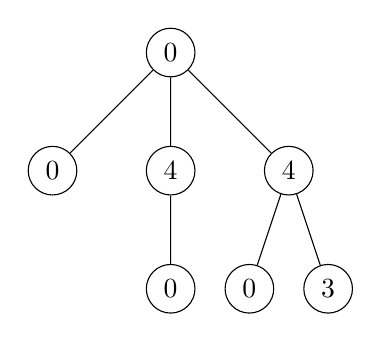
\begin{tikzpicture}[scale=1, transform shape]
\tikzstyle{level 2}=[sibling distance=10mm]
    \node [circle, draw] (z){$0$}
        child {node [circle, draw] (a) {$0$}}
        child {node [circle, draw] (d) {$4$}
            child {node [circle, draw] (g) {$0$}}
        }
        child {node [circle, draw] (b) {$4$}
            child {node [circle, draw] (e) {$0$}}
            child {node [circle, draw] (f) {$3$}}
        };
\end{tikzpicture}

\begin{lstlisting}
def replace_x(t, x):
    







\end{lstlisting}

\begin{solution}
\begin{lstlisting}
   new_label = label(t)
   if new_label == x:
        new_label = 0
   new_branches = [replace_x(b, x) for b in branches(t)]
   return tree(new_label, new_branches)
\end{lstlisting}
\end{solution}
\end{blocksection}
